\newpage % Rozdziały zaczynamy od nowej strony.
\subsection{Hetionet knowledge graph}
\label{subsec:benchmark-endpoint}

Task~B is evaluated on a benchmark dataset derived from Hetionet. 
Hetionet is a heterogeneous network
(\emph{hetnet}) that integrates biomedical knowledge from 29 publicly
available resources. It represents biological and pharmacological entities
as nodes and documented relationships between them as typed edges.

Hetionet v1.0 contains 47{,}031 nodes belonging to 11 node types and
2{,}250{,}197 relationships of 24 types. The graph includes compounds,
diseases, genes, anatomies, pathways, biological processes, molecular
functions, cellular components, pharmacologic classes, side effects, and
symptoms. This heterogeneous structure makes Hetionet suitable for node classification task described further. 
The details of benchmark check are included in Section ~\ref{subsec:benchmark-endpoint}.

\begin{figure}[h]
    \centering
    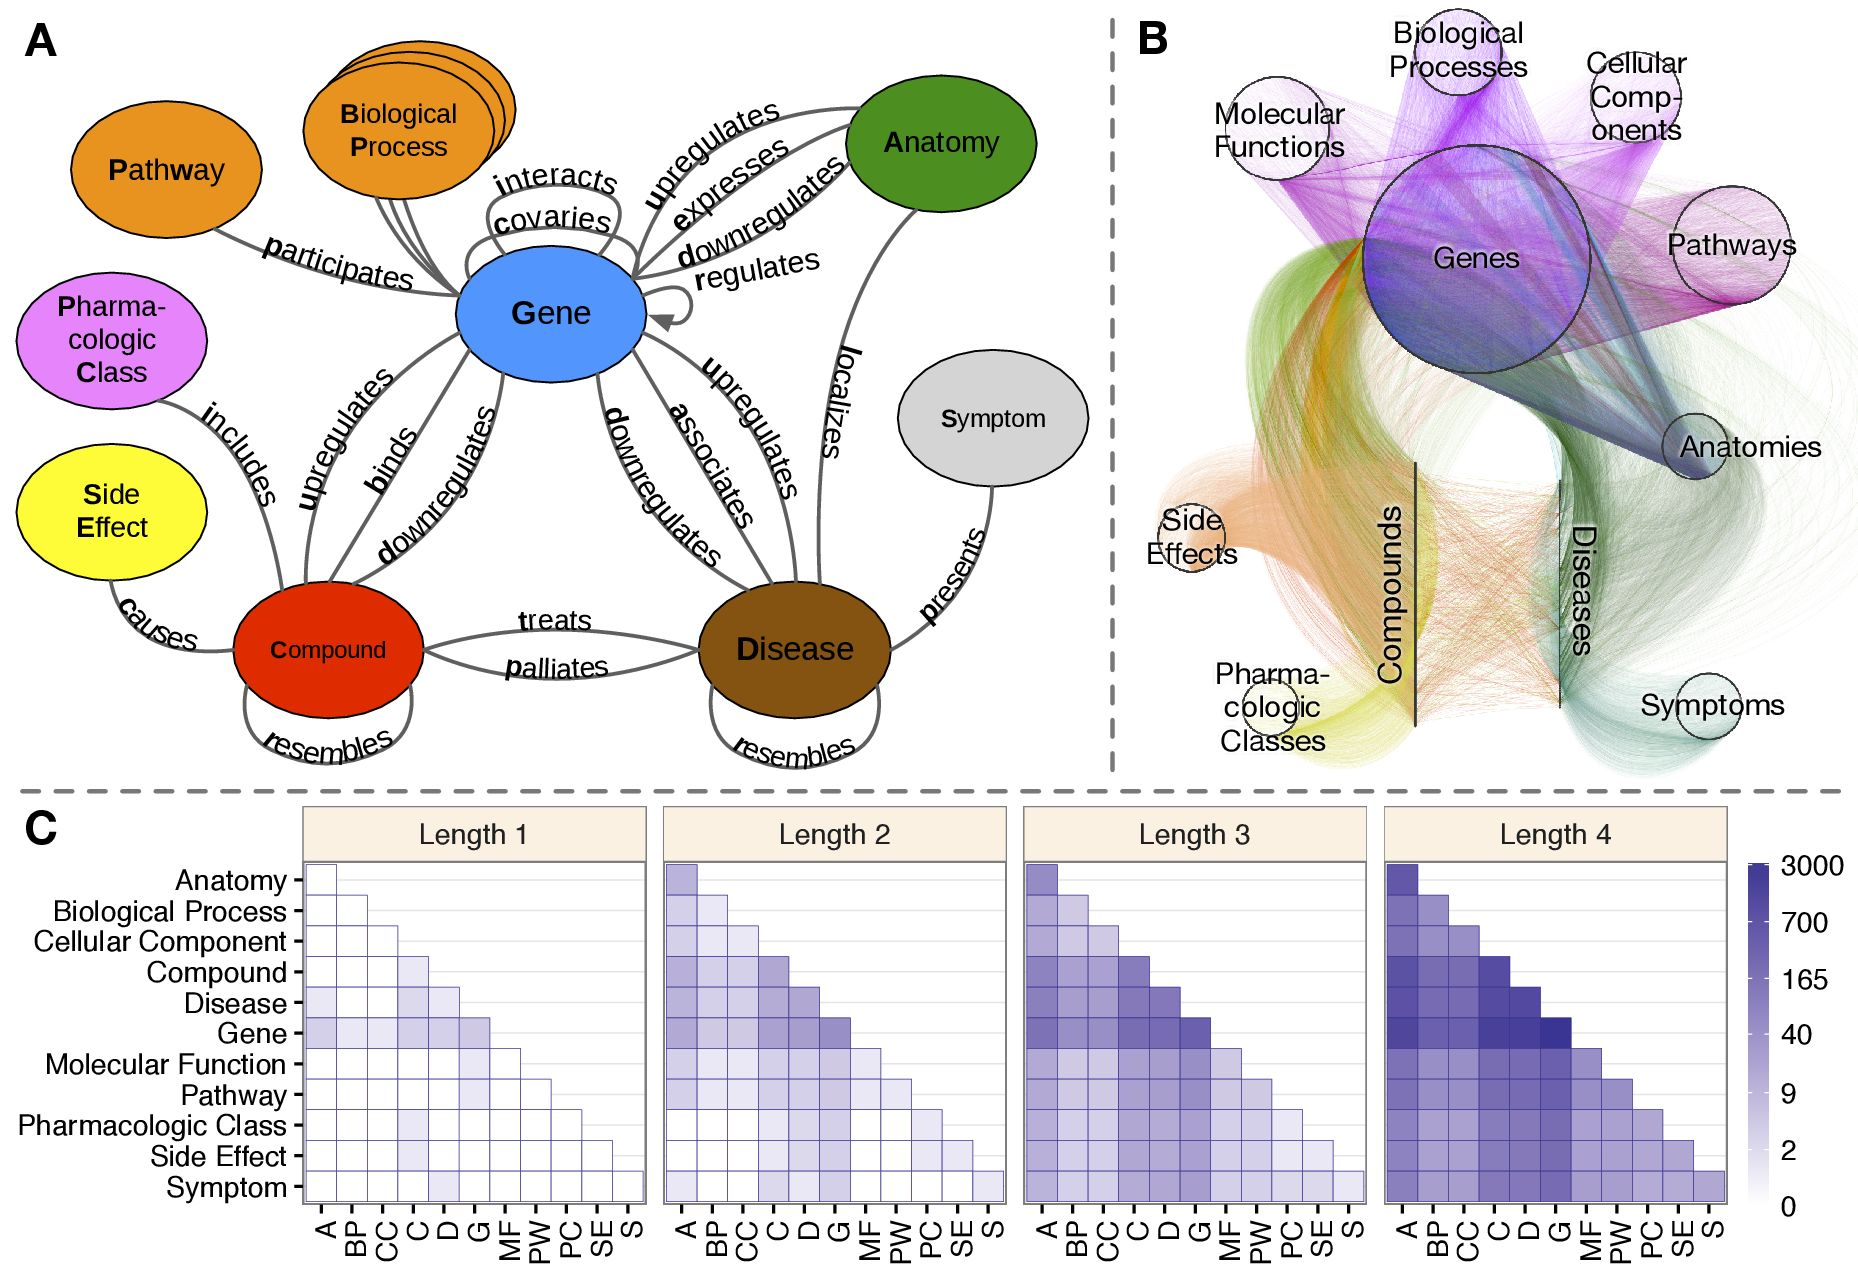
\includegraphics[width=\textwidth, height=0.45\textheight, keepaspectratio]{rysunki/elife-26726-fig1-v2.jpg}
    \caption{Hetionet knowledge graph}
    \label{fig:hetionet-original}
\end{figure}
Figure~\ref{fig:hetionet-original} shows the Hetionet v1.0 network structure.\footnote{Source: \url{https://www.researchgate.net/figure/Hetionet-v10-A-The-metagraph-a-schema-of-the-network-types-B-The-hetnet-visualized_fig1_345109349}}
Hetionet was selected because it is heterogeneous and supports a
multi-label prediction setup analogous to the synthetic
task. 


\subsubsection{Data Representation}

The
benchmark on this datasetis a structural proxy---the
pipeline, layer slots, and statistical evidence branch are reused, but the graph is
reconstructed to resemble the synthetic schema in topology. 
Below  are listed reconstruction steps taken. 

\begin{enumerate}[label=(\roman*)]
  \item \textbf{Instance.} A compound takes the role of the patient: the
    topology is shared and a compound is described by the edges linking it to
    the remaining entities. A compound is therefore \emph{not} a node of the
    graph, which means an entity can serve as a feature column only if it
    connects to compounds directly.

  \item \textbf{Target.} The predicted endpoint is a disease node, labelled positive when a
  \texttt{treats} or \texttt{palliates} edge links the compound to that disease
  (the two relations were merged).
  Prevalences range from $1.29\%$ to $4.51\%$ over the twenty most frequent
  diseases. 

  \item \textbf{Layer mapping.} Node types were mapped onto the slots of the
    synthetic schema as presented in \cref{tab:hetionet-mapping}.

  \item \textbf{Direction.} Hetionet edges are undirected associations.
    For pipeline compatibility, every retained edge was oriented from the
    lower to the higher synthetic layer and intra-layer edges were
    discarded, guaranteeing acyclicity. 

  \item \textbf{Path length.} Two changes lengthen the paths to a disease. First, a pathway and
  biological-process layer was inserted as the third layer, while the direct
  \texttt{DaG} edges were kept. Second, class-to-gene edges were added, because
  pharmacologic classes connect only to compounds in Hetionet and would otherwise
  have no edges at all. Such an edge is created when at least three training
  compounds of a class bind the same gene.

\end{enumerate}

% =====================================================================
%  Mapping of Hetionet node types onto the layers of the synthetic schema.
%  PREAMBLE: \usepackage{booktabs}\usepackage{tabularx}\usepackage{array}
% =====================================================================
\begin{table}[htbp]
  \centering
  \small
  \caption{Mapping of Hetionet entities onto the synthetic layer schema.}
  \label{tab:hetionet-mapping}
  \begin{tabular}{clll}
    \toprule
    Layer & Slot & Hetionet entity & Observed \\
    \midrule
    1 & \texttt{patient\_context}            & Pharmacologic Class (filtered)   & yes \\
    2 & \texttt{drug\_exposure}              & Gene, bound (\texttt{CbG})       & yes \\
    3 & \texttt{mechanism}                   & Pathway, Biological Process      & no (latent) \\
    4 & \texttt{adr\_or\_intermediate\_state} & Gene, associated (\texttt{DaG}) & no (latent) \\
    5 & \texttt{clinical\_endpoint}          & Disease                          & target \\
    \bottomrule
  \end{tabular}
\end{table}

In \cref{fig:updated_hetionet} there is presented the updated view of graph. 


\begin{figure}[htbp]
  \centering
  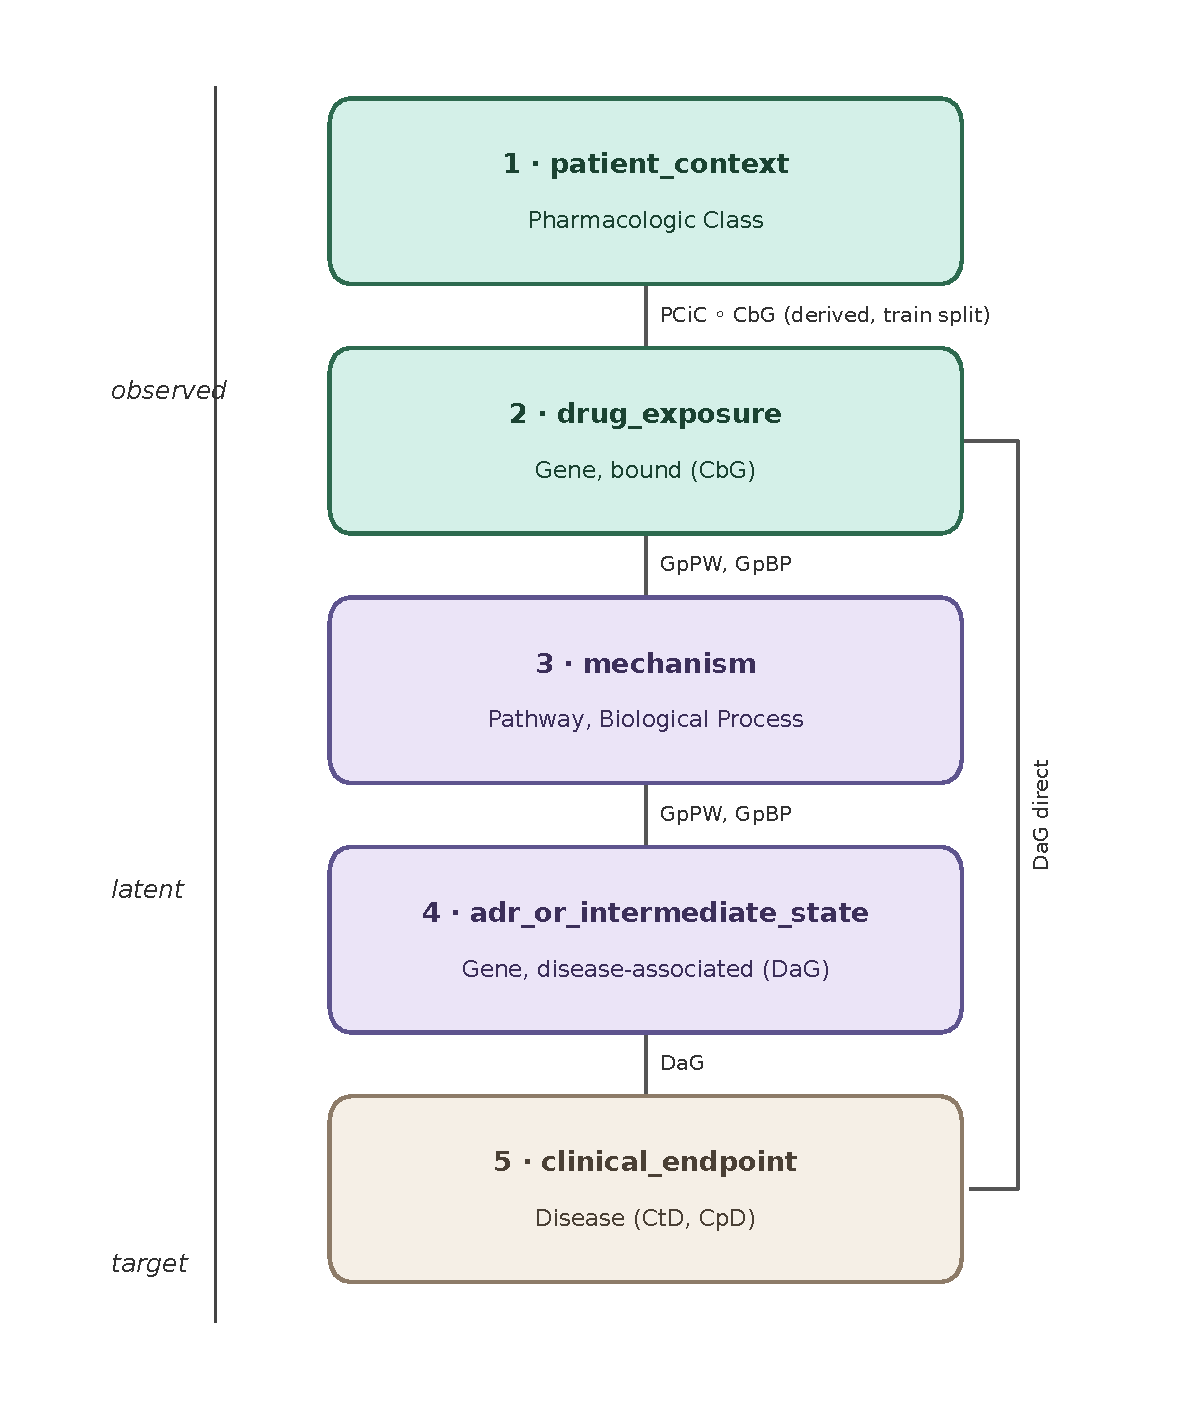
\includegraphics[width=0.92\textwidth,keepaspectratio]{rysunki/hetionet_layer_mapping.pdf}
  \caption{Hetionet layer mapping after reconstruction onto the synthetic schema.}
  \label{fig:updated_hetionet}
\end{figure}



\subsubsection{Results}

% The models on benchmark dataset shows the same trend as on synthethic dataset. 
% The approach with HCR significantly improves results comparing to baseline model without HCR. 
% It generates similar results as models with residual connections, but what it is interesting on the benchamrk dataset
% HCR combined with residual connections reaches the higher results than separated approach. 

The benchmark reproduces several trends
observed on the synthetic dataset---depth sensitivity without stabilisers,
partial recovery with HCR---under a different graph semantics and without
oracle metrics. The gain from HCR is conditional on the state of the
propagation path: at $L=6$ without
residual connections the baseline collapses to $0.585$ AUC on test, while every
HCR variant recovers a substantial part of it, up to $0.757$ for
\emph{typed+triple}. At $L=1$, where the receptive field of an endpoint
coincides with the input of the HCR branch, no variant improves on the
baseline, and the concatenated variants are slightly worse.

In the benchmark dataset, residual connections and HCR combine additively at
$L=6$. The baseline
reaches $0.585$ without either mechanism, $0.680$--$0.757$ with HCR alone,
$0.728$ with residual alone, and $0.760$ with both. The combination is
therefore better than either component in isolation.

The reason is the structure of the two graphs. In the synthetic graph the direct
parents of an endpoint are observed, so the statistical evidence branch and the one-hop
receptive field read the same variables and the two mechanisms address the same
bottleneck. In the Hetionet-derived graph depth is more crucial because some
layers are latent. Information must
therefore traverse several hops, and the residual path and the HCR bypass
contribute at different points of that route.

Overall, the proxy experiment suggests that combining message passing
with the statistical evidence branch remains useful with 
multi-hop reasoning. Whether an
additional residual path helps or hinders depends on where 
the statistical
evidence enters the model.


% =====================================================================
%  PROXY DATASET RESULTS (Hetionet, cut A, proxy3_clean)
%  1552 compounds, 20 endpoints, seed 42, conv_type = transformer,
%  hidden = 64, batch = 8, lr = 1e-3, dropedge = 0.0
% =====================================================================
\begin{table}[H]
  \centering
  \small
  \setlength{\tabcolsep}{4pt}
  \caption{Benchmark results for endpoint prediction.}
  \label{tab:proxy-full}
  \sisetup{table-format=1.3}
  \begin{tabular}{ccl SSS SSS}
    \toprule
    & & & \multicolumn{3}{c}{Validation} & \multicolumn{3}{c}{Test} \\
    \cmidrule(lr){4-6}\cmidrule(lr){7-9}
    $L$ & Res. & HCR & {AUC} & {AP} & {Lift} & {AUC} & {AP} & {Lift} \\
    \midrule
    1 & no  & ---              & 0.757 & 0.188 & 7.92  & 0.664 & 0.120 & 6.49 \\
    1 & no  & nonlin.\ bin.    & 0.763 & 0.207 & 8.75  & 0.657 & 0.120 & 6.47 \\
    1 & no  & nonlin.\ all     & 0.761 & 0.206 & 8.69  & 0.665 & 0.140 & 7.55 \\
    1 & no  & typed+triple     & 0.765 & 0.160 & 6.75  & 0.662 & 0.104 & 5.63 \\
    \addlinespace[2pt]
    1 & yes & ---              & 0.756 & 0.196 & 8.26  & 0.669 & 0.106 & 5.72 \\
    1 & yes & nonlin.\ bin.    & 0.756 & 0.201 & 8.49  & 0.670 & 0.135 & 7.31 \\
    1 & yes & nonlin.\ all     & 0.758 & 0.206 & 8.69  & 0.664 & 0.135 & 7.32 \\
    1 & yes & typed+triple     & 0.750 & 0.157 & 6.61  & 0.661 & 0.098 & 5.30 \\
    \midrule
    2 & no  & nonlin.\ all     & 0.763 & 0.263 & 11.10 & 0.694 & 0.173 & 9.34 \\
    2 & no  & typed+triple     & 0.778 & 0.263 & 11.10 & 0.677 & 0.175 & 9.46 \\
    \addlinespace[2pt]
    2 & yes & nonlin.\ all     & 0.760 & 0.224 & 9.44  & 0.684 & 0.154 & 8.31 \\
    2 & yes & typed+triple     & 0.765 & 0.232 & 9.79  & 0.690 & 0.174 & 9.43 \\
    \midrule
    3 & no  & ---              & 0.756 & 0.199 & 8.38  & 0.722 & 0.152 & 8.24 \\
    3 & no  & nonlin.\ bin.    & 0.805 & 0.275 & 11.62 & 0.686 & 0.169 & 9.14 \\
    3 & no  & nonlin.\ all     & 0.800 & 0.259 & 10.91 & 0.700 & 0.166 & 8.99 \\
    3 & no  & typed+triple     & 0.794 & 0.237 & 10.01 & 0.702 & 0.168 & 9.11 \\
    \addlinespace[2pt]
    3 & yes & ---              & 0.799 & 0.225 & 9.48  & 0.685 & 0.166 & 8.97 \\
    3 & yes & nonlin.\ bin.    & 0.814 & 0.235 & 9.90  & 0.714 & 0.183 & 9.92 \\
    3 & yes & nonlin.\ all     & 0.807 & 0.259 & 10.91 & 0.677 & 0.174 & 9.39 \\
    3 & yes & typed+triple     & 0.805 & 0.248 & 10.45 & 0.708 & 0.180 & 9.72 \\
    \midrule
    4 & no  & nonlin.\ all     & 0.757 & 0.230 & 9.70  & 0.678 & 0.151 & 8.14 \\
    4 & no  & typed+triple     & 0.807 & 0.262 & 11.06 & 0.747 & 0.181 & 9.79 \\
    \addlinespace[2pt]
    4 & yes & nonlin.\ all     & 0.814 & 0.238 & 10.05 & 0.715 & 0.180 & 9.76 \\
    4 & yes & typed+triple     & 0.806 & 0.240 & 10.12 & 0.713 & 0.168 & 9.06 \\
    \midrule
    5 & no  & nonlin.\ all     & 0.783 & 0.239 & 10.08 & 0.680 & 0.158 & 8.52 \\
    5 & no  & typed+triple     & 0.807 & 0.246 & 10.37 & 0.746 & 0.163 & 8.84 \\
    \addlinespace[2pt]
    5 & yes & nonlin.\ all     & 0.815 & 0.291 & 12.29 & 0.727 & 0.179 & 9.71 \\
    5 & yes & typed+triple     & 0.813 & 0.270 & 11.37 & 0.724 & 0.211 & 11.41 \\
    \midrule
    6 & no  & ---              & 0.610 & 0.121 & 5.11  & 0.585 & 0.077 & 4.14 \\
    6 & no  & nonlin.\ bin.    & 0.782 & 0.210 & 8.86  & 0.680 & 0.174 & 9.42 \\
    6 & no  & nonlin.\ all     & 0.794 & 0.237 & 9.99  & 0.682 & 0.157 & 8.51 \\
    6 & no  & typed+triple     & 0.803 & 0.263 & 11.11 & 0.757 & 0.175 & 9.45 \\
    \addlinespace[2pt]
    6 & yes & ---              & 0.817 & 0.255 & 10.77 & 0.728 & 0.173 & 9.36 \\
    6 & yes & nonlin.\ bin.    & 0.832 & 0.310 & 13.06 & 0.760 & 0.179 & 9.70 \\
    6 & yes & nonlin.\ all     & 0.812 & 0.235 & 9.92  & 0.734 & 0.166 & 8.96 \\
    6 & yes & typed+triple     & 0.808 & 0.251 & 10.59 & 0.730 & 0.205 & 11.10 \\
    \bottomrule
  \end{tabular}
\end{table}


% ---------------------------------------------------------------------
% TABLE 1 - full observability regime
% ---------------------------------------------------------------------
% \begin{table}[H]
%     \centering
%     \caption{Results under full observability on the proxy dataset. The
%       epoch was selected on the validation set. \texttt{---} in the HCR
%       column denotes a model without the HCR branch. Lift is AUPRC
%       divided by the prevalence baseline. Jumping knowledge was not used
%       in any configuration.}
%     \label{tab:proxy-full}
%     \sisetup{table-format=1.3}
%     \begin{tabular}{ccl SSS SSS}
%       \toprule
%       & & & \multicolumn{3}{c}{Validation} & \multicolumn{3}{c}{Test} \\
%       \cmidrule(lr){4-6}\cmidrule(lr){7-9}
%       $L$ & Residual & HCR & {AUC} & {AUPRC} & {Lift} & {AUC} & {AUPRC} & {Lift} \\
%       \midrule
%       1 & no  & ---            & 0.757 & 0.188 & 7.92  & 0.664 & 0.120 & 6.49 \\
%       1 & no  & nonlin.\ 9D    & 0.763 & 0.207 & 8.75  & 0.657 & 0.120 & 6.47 \\
%       1 & no  & typed 41D      & 0.759 & 0.194 & 8.17  & 0.663 & 0.116 & 6.29 \\
%       \addlinespace[2pt]
%       1 & yes & ---            & 0.756 & 0.196 & 8.26  & 0.669 & 0.106 & 5.72 \\
%       1 & yes & nonlin.\ 9D    & 0.756 & 0.201 & 8.49  & 0.670 & 0.135 & 7.31 \\
%       1 & yes & typed 41D      & 0.754 & 0.185 & 7.79  & 0.671 & 0.124 & 6.71 \\
%       \midrule
%       3 & no  & ---            & 0.756 & 0.199 & 8.38  & {\bfseries 0.722} & 0.152 & 8.24 \\
%       3 & no  & nonlin.\ 9D    & 0.805 & 0.275 & 11.62 & 0.686 & 0.169 & 9.14 \\
%       3 & no  & typed 41D      & 0.812 & 0.243 & 10.26 & 0.678 & 0.154 & 8.32 \\
%       \addlinespace[2pt]
%       3 & yes & ---            & 0.799 & 0.225 & 9.48  & 0.685 & 0.166 & 8.97 \\
%       3 & yes & nonlin.\ 9D    & 0.814 & 0.235 & 9.90  & 0.714 & 0.183 & 9.92 \\
%       3 & yes & typed 41D      & 0.802 & 0.255 & 10.76 & 0.678 & 0.151 & 8.16 \\
%       \midrule
%       6 & no  & ---            & 0.610 & 0.121 & 5.11  & 0.585 & 0.077 & 4.14 \\
%       6 & no  & nonlin.\ 9D    & 0.782 & 0.210 & 8.86  & 0.680 & 0.174 & 9.42 \\
%       6 & no  & typed 41D      & 0.794 & 0.235 & 9.89  & 0.680 & 0.126 & 6.84 \\
%       \addlinespace[2pt]
%       6 & yes & ---            & 0.817 & 0.255 & 10.77 & 0.728 & 0.173 & 9.36 \\
%       6 & yes & nonlin.\ 9D    & {\bfseries 0.832} & {\bfseries 0.310} & {\bfseries 13.06} & {\bfseries 0.760} & 0.179 & 9.70 \\
%       6 & yes & typed 41D      & 0.815 & 0.284 & 11.99 & 0.744 & {\bfseries 0.239} & {\bfseries 12.91} \\
%       \bottomrule
%     \end{tabular}
%   \end{table}
  
  
  % ---------------------------------------------------------------------
  % TABLE 3 - representation smoothing metrics
  % ---------------------------------------------------------------------
  % \begin{table}[H]
  %   \centering
  %   \caption{Representation smoothing metrics under full observability,
  %     measured on the validation set. By the conventional reading, lower
  %     MAD and higher cosine similarity indicate stronger smoothing.
  %     Validation AUC is repeated for comparison. Note that residual
  %     configurations appear more smoothed by every metric while
  %     performing better.}
  %   \label{tab:proxy-oversmoothing}
  %   \sisetup{table-format=1.4}
  %   \begin{tabular}{ccl SSSS S[table-format=1.3]}
  %     \toprule
  %     $L$ & Residual & HCR & {MAD} & {Cos.\ sim.} & {Cos.\ sim.\ (ep.)} & {Dirichlet} & {AUC} \\
  %     \midrule
  %     1 & no  & ---         & 0.7691 & 0.6216 & 0.8246 & 0.2706 & 0.757 \\
  %     1 & no  & nonlin.\ 9D & 0.7629 & 0.6142 & 0.7844 & 0.2495 & 0.763 \\
  %     1 & no  & typed 41D   & 0.7684 & 0.6191 & 0.8148 & 0.2706 & 0.759 \\
  %     \addlinespace[2pt]
  %     1 & yes & ---         & 0.7363 & 0.7042 & 0.7606 & 0.5724 & 0.756 \\
  %     1 & yes & nonlin.\ 9D & 0.7448 & 0.6946 & 0.7060 & 0.5048 & 0.756 \\
  %     1 & yes & typed 41D   & 0.7410 & 0.7026 & 0.7899 & 0.5022 & 0.754 \\
  %     \midrule
  %     3 & no  & ---         & 0.6515 & 0.6798 & 0.9582 & 0.1175 & 0.756 \\
  %     3 & no  & nonlin.\ 9D & 0.7067 & 0.6641 & 0.8365 & 0.0904 & 0.805 \\
  %     3 & no  & typed 41D   & 0.7235 & 0.6314 & 0.7333 & 0.0972 & 0.812 \\
  %     \addlinespace[2pt]
  %     3 & yes & ---         & 0.4842 & 0.8319 & 0.7772 & 0.3712 & 0.799 \\
  %     3 & yes & nonlin.\ 9D & 0.5517 & 0.7782 & 0.7752 & 0.3905 & 0.814 \\
  %     3 & yes & typed 41D   & 0.5113 & 0.8275 & 0.7132 & 0.4044 & 0.802 \\
  %     \midrule
  %     6 & no  & ---         & 0.7060 & 0.6530 & 0.8604 & 0.1024 & 0.610 \\
  %     6 & no  & nonlin.\ 9D & 0.7101 & 0.6495 & 0.7815 & 0.0892 & 0.782 \\
  %     6 & no  & typed 41D   & 0.7222 & 0.6408 & 0.8657 & 0.0949 & 0.794 \\
  %     \addlinespace[2pt]
  %     6 & yes & ---         & 0.5634 & 0.7975 & 0.7949 & 0.3143 & 0.817 \\
  %     6 & yes & nonlin.\ 9D & 0.5030 & 0.8174 & 0.6658 & 0.2636 & 0.832 \\
  %     6 & yes & typed 41D   & 0.5623 & 0.8095 & 0.8472 & 0.3930 & 0.815 \\
  %     \bottomrule
  %   \end{tabular}
  % \end{table}